\documentclass[12pt,a4paper]{article}

\usepackage[english]{babel}
\usepackage{hyperref}
\usepackage{graphicx}
\usepackage{nicefrac}
\usepackage{caption}

%% The title of your survey
\title{ Survey of mobile network security in trending technologies, focusing on Bluetooth and NFC }

%% Both authors
\author{ Johannes Kurz \\
         e0727957 \\%student ID
         \and
         Gerhard Schraml \\
         e0728067 % student ID
}
\date{\today}

%% The actual contents of the document
\begin{document}

%% Generate the title
\maketitle

%% Write the abstract  
%% ----------------------------------------------------------------------------
\begin{abstract}
\noindent
Write a short abstract about the topics contained in the paper. This is usually the last step to do.
\end{abstract}


%% Introduction
%% ----------------------------------------------------------------------------
\section{Introduction}

\begin{table}
\begin{tabular}{r|l}
\hline
\multicolumn{2}{c}{paper structure proposal} \\
\hline
1 - 1\nicefrac{1}{2} page & title + abstract + introduction \\
1 page & mobile networks security basics general \\
\nicefrac{1}{2} page & nfc general description \\
\nicefrac{1}{2} page & nfc threat introduction and listing \\
3 - 5 pages & nfc threats in detail (1 page per threat?) + solution \\
4 - 6 pages & bluetooth TODO shorty \\
\nicefrac{1}{2} page & conclusion \\
1 - 2 pages & references \\
\hline \hline
11\nicefrac{1}{2} - 17 pages & total \\
\hline \hline
\end{tabular}
\end{table}

What you should include in the introduction
\begin{itemize}
 \item Describe the topic (Importance, Significance)
 \item Give a summary of the surveyed topic
\end{itemize}


%% Actual Survey Work
%% ----------------------------------------------------------------------------
%% You can introduce further sections as well
\section{Mobile Networks Security Basics General whatever}

\section{Security in Near Field Communication}

\subsection{Terms and general description}

More and more people world wide start using \emph{Near Field Communication} (NFC) for personal purposes. Goal of the technology is the convenient transfer of small amounts of data by just simply wiping compatible devices over each others. As the communication is contactless, bringing sender and receiver to close proximity suffices to establishing a connection. Usually the working distance for NFC connections does not exceed about 10 to 20 centimeters. The technology is based upon \emph{Radio-Frequency Identification} (RFID) - it 	similarly uses electromagnetic radiation for transporting signals over small distances. Therefor a small magnetic field is established with the purpose of bridging the physical space between participating devices.

Basically two types of NFC devices exist. \emph{Active devices} take care of the establishment of the necessary magnetic field. As this is an energy-consuming task, they are usually connected to a power supply. \emph{Passive devices} normally don't possess a built-in power supply. They make use of small amounts of power they are able to harvest from the magnetic field issued by a connected active device. Hence, passive devices are idle when there is no connection present. Typical examples for such devices are so-called NFC tags, e.g. containing additional information about an exhibit in a museum where it is attached to. A user could then easily access this information by hovering its NFC-enabled electronic device, capable of reading the NFC tag, over it.

Mobile devices can choose out of three different communication modes. In \emph{Peer-To-Peer} mode, two active NFC-enabled devices communicate on an equal basis. Usually the task of emitting the necessary magnetic field is carried out in an alternating way by both participants. In \emph{Reader/Writer} mode an active device is reading data from respectively writing data to passive NFC tags. Finally, in \emph{Card Emulation} mode a mobile device is acting as NFC tag allowing other (active) devices to read information from it. This mode is mostly used for electronic ticketing or contactless payment applications using mobile phones.

\subsection{Selected security threats}
 
bar bar foo foo einführender text ein paar zeilen was es nicht alles gibt bar bar foo foo bar bar foo foo bar bar foo foo bar bar foo foo

\subsubsection{Smart Poster Spoofing}

Typically, NFC communication between mobile devices and tags (or other devices) uses the \emph{NFC Data Exchange Format (NDEF)}. It is defined by the NFC Forum\footnote{\url{www.nfc-forum.org}}, a standardization organisation in the area of NFC. The NDEF format consists of several record data types, headed by \emph{Text}, \emph{URI} and \emph{Smart Poster} record types.\cite{DBLP:conf/IEEEares/Mulliner09} 

Text records simply contain an arbitrary, human-readable text, optionally followed by a language identifier.

URI records include a URI of arbitrary protocol pointing to further information or an action to perform. Based on the protocol, e.g. HTTP, TEL, SMS, MAILTO, the receiving device determines the target application to deal with the given URI. Thus the NFC subsystem of a device can be seen as kind of a job dispatcher.

Smart Poster records usually consist of a text record, containing the title or short description of a hovered NFC tag, and a URI record pointing to some more detailed information on the item the tag is attached to. One proper use case is, as already mentioned above, to provide further information on museum exhibits by just hovering the attached NFC tag.

\paragraph{Manipulating the content of a Smart Poster}

In \cite{DBLP:conf/IEEEares/Mulliner09}, a way of tricking users into acknowledging actions, they actually don't want to perform, is presented. One could physically replace smart tags with new ones containing malicious information. Due to limitations of a smart phone device, expected information is shown at the display of a victims device, while the underlying action e.g. links to an attackers site. In the test, a Nokia 6131 device was used, which would display only the text content of a Smart Poster if it exceeds the screen size. Thus, the transported URI is, at least at first sight, not presented to the user. Figure \ref{img_smart_poster_spoofing} shows an example of how such a spoofed message could be constructed. Another example is the abuse of the TEL protocol issuing a phone call. The attacker could display a trusted phone number while actually attaching a premium rate number leading to unwanted expenses for the victim.

\begin{figure}[h]
\begin{center}
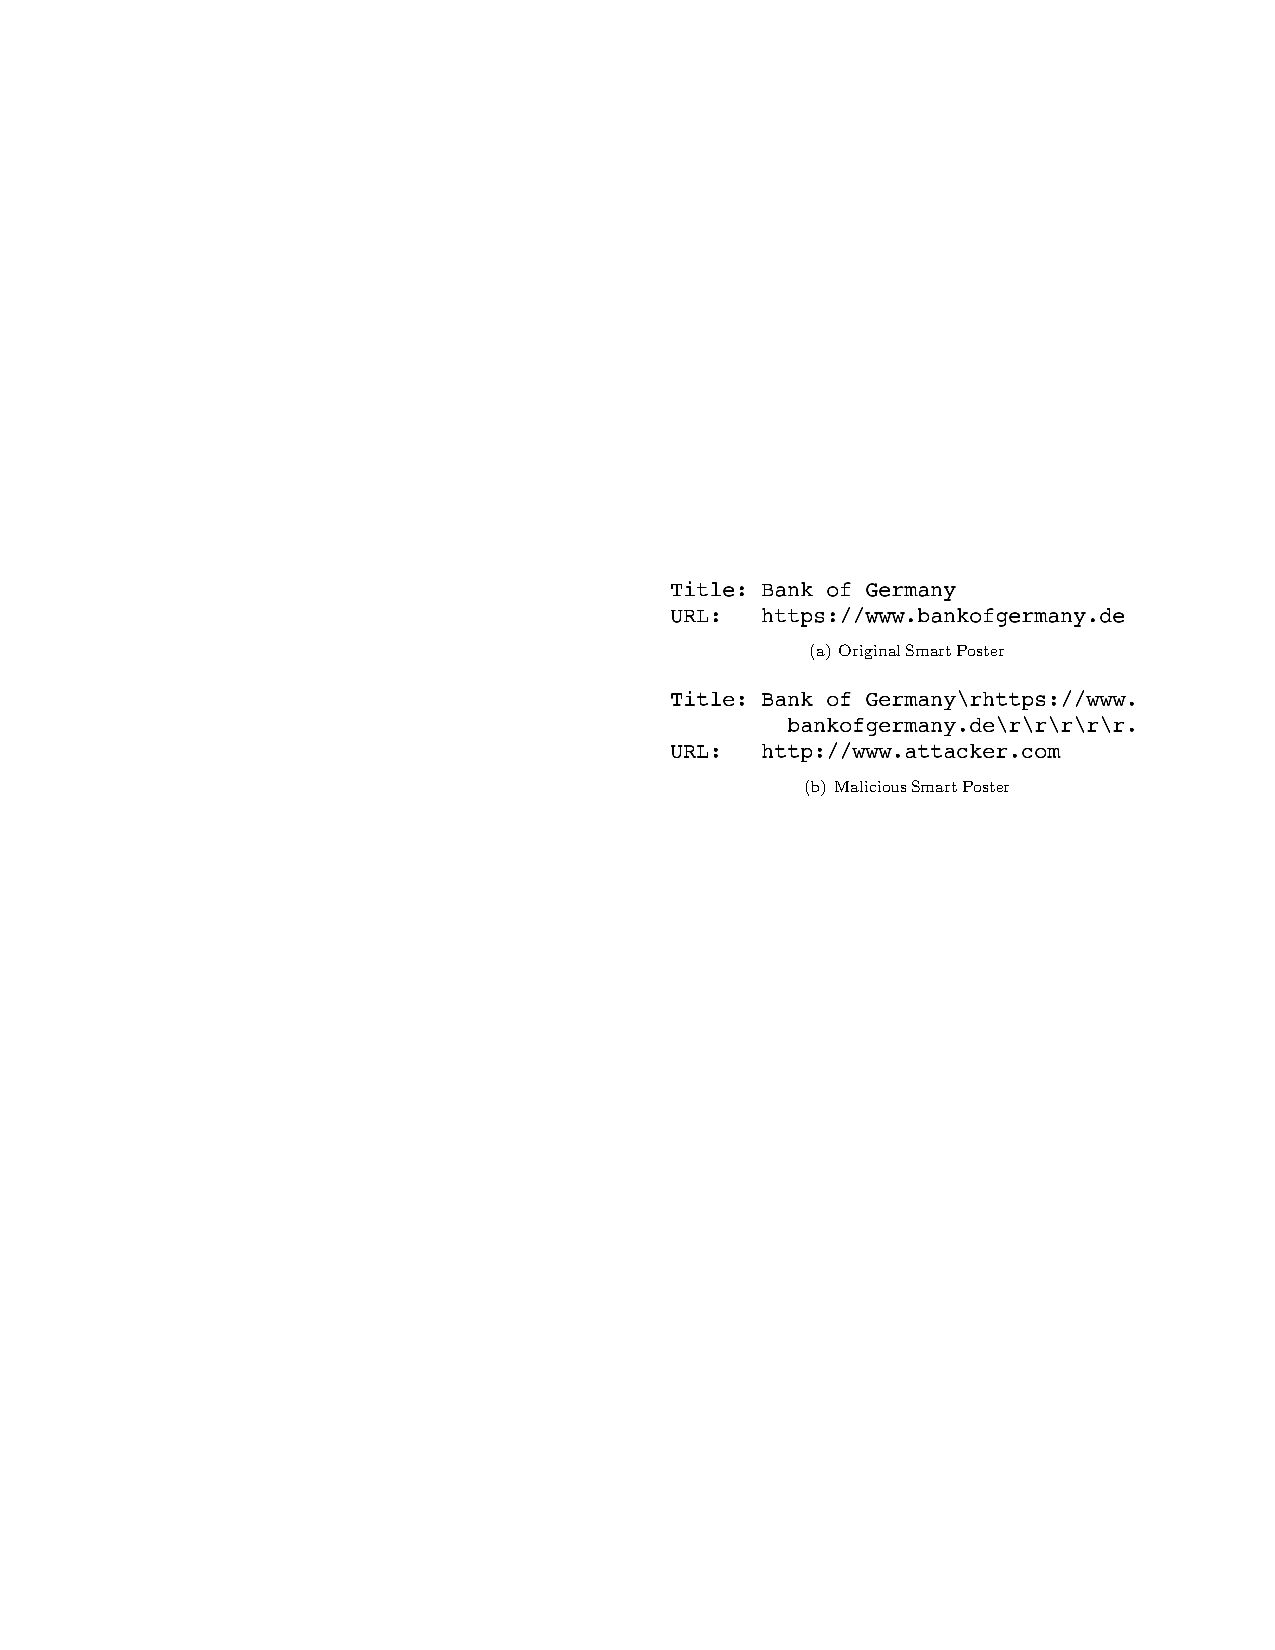
\includegraphics{img/smart_poster_spoofing}
\caption{Smart Poster Spoofing Example\cite{DBLP:conf/IEEEares/Mulliner09}}
\label{img_smart_poster_spoofing}
\end{center}
\end{figure}

\paragraph{Countermeasures against Smart Poster Spoofing}

\cite{DBLP:conf/wowmom/WuQKKT12} presents S-SPAN, a system aiming at securing the use of Smart Poster reads from NFC tags. Basic approach is not to store the actual information in plain text on the NFC tag. The tag rather contains a non-guessable and non-human-readable identifier which is used to locate the Smart Poster contents in a online database. The user of the mobile device has to be logged into the online database when touching the NFC tag. Over secured connection, the database is queried for the identifier and replies with the actuals contents. The contents of the database are administered by the owner of the smart tag. Identifiers are never used twice to prevent accidental usage of old tags. Consequently, Smart Poster can expire at some time. The approach entails better security as actual URIs are always retrieved by a trusted entity. On the other hand, additional latency has to be accepted for querying the database.

\cite{DBLP:conf/trustcom/HameedHHK14} refers to the latency problem of S-SPAN and presents a "Lightweight Security Middleware to Detect Malicious Content in NFC Tags or Smart Posters". The proposed middleware is run between the NFC controller and the application layer of the device and takes care of all Smart Poster tag reads. In contrast to S-SPAN, data (Text and URI) is directly stored on the tag. The middleware, depicted in figure \ref{img_lightweight_security_middleware}, performs a series of checks against the delivered URI. First, a \emph{white list} is queried against the URI. If the given URI can be found, the Smart Poster is directly forwarded to the application layer. If not, a \emph{black list} approach is performed. If the URI is blacklisted, the middleware prompts the user to decide on whether to continue reading the Smart Poster. If the URI is not blacklisted, a final validation attempt is made by querying \emph{Crowd-sourced Internet Website Reputation Ratings}. When the query results in a predefined minimum reputation score, the Smart Poster again is forwarded. Performance observations show, that white- and blacklist hits cause very low latency, while reputation querying takes a maximum of 1 second in the given test environment.

\begin{figure}[h]
\begin{center}
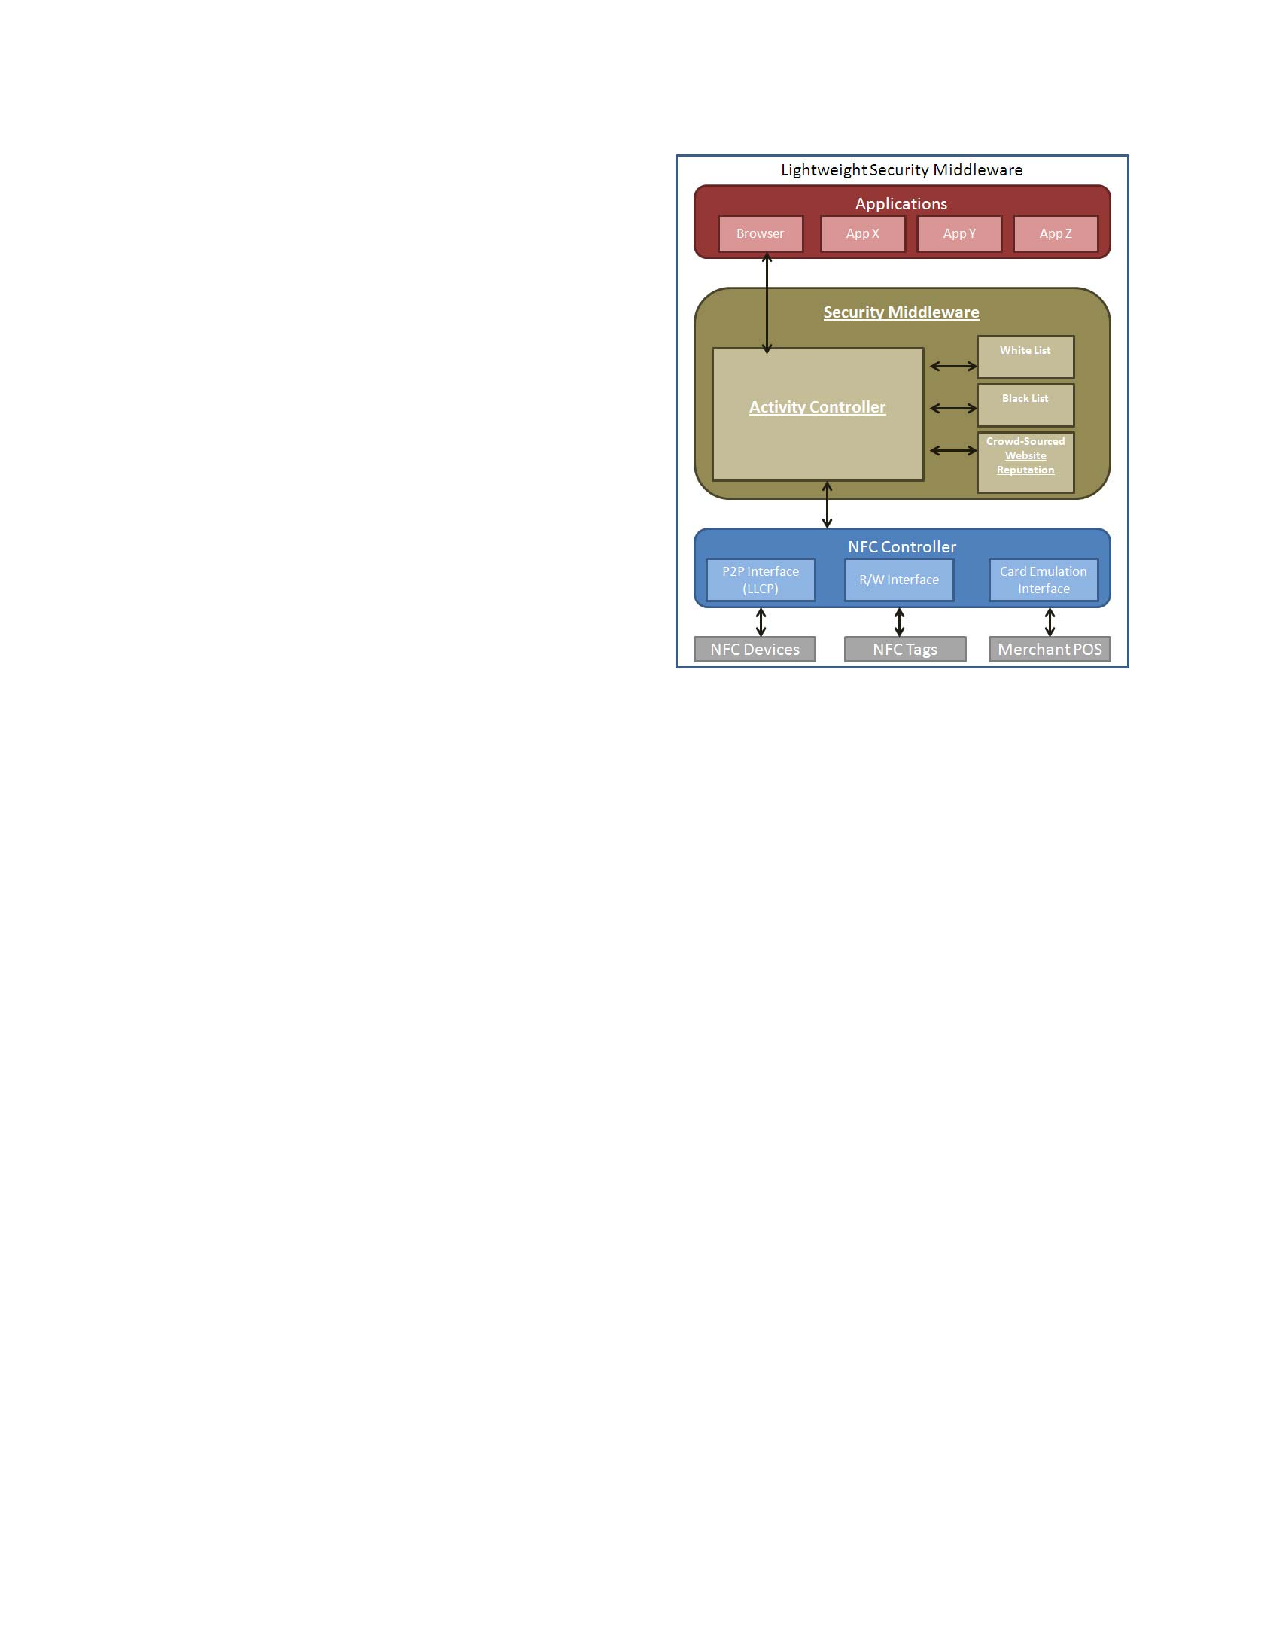
\includegraphics{img/lightweight_security_middleware}
\caption{NFC application architecture from \cite{DBLP:conf/trustcom/HameedHHK14}}
\label{img_lightweight_security_middleware}
\end{center}
\end{figure}

\subsubsection{Eavesdropping}

threat description and possible solution (\emph{nShield}) \cite{DBLP:conf/mobisys/ZhouX14}

bar bar foo foo

\subsubsection{Relay attacks}

TODO man-in-the-middle? more general than relay attacks?

Problem description, practical implementations and countermeasures \cite{DBLP:journals/compsec/HanckeMM09} \cite{DBLP:conf/rfidsec/FrancisHMM10} \cite{DBLP:conf/sec/RolandLS12}

bar bar foo foo

\subsubsection{Signal jamming}

\emph{EnGarde} - rule based signal jamming as a protection mechanism \cite{DBLP:conf/mobisys/GummesonPGTZ13}

TODO denial of service? = basically just jamming the signal

bar bar foo foo

\section{Security in Bluetooth communications}

%% Conclusion
%% ----------------------------------------------------------------------------
\section{Conclusion}
Put your conclusion about the topic here



%% References 
%% ----------------------------------------------------------------------------
\bibliography{references}{}
\bibliographystyle{plain}
\end{document}

